\documentclass[11pt]{article}
\usepackage[spanish]{babel}
\usepackage[utf8]{inputenc}
\usepackage{amsmath}
\usepackage{geometry}
\usepackage{graphicx}
\usepackage{listings}
\usepackage{xcolor}
\usepackage{float}
\graphicspath{{images/}}
\geometry{margin=2.5cm}

\newcommand{\Sen}{\operatorname{Sen}}
\newcommand{\Cos}{\operatorname{Cos}}

\definecolor{matlabkeyword}{rgb}{0,0,1}
\definecolor{matlabcomment}{rgb}{0.13,0.55,0.13}
\definecolor{matlabstring}{rgb}{0.63,0.13,0.94}
\definecolor{matlabbg}{rgb}{0.97,0.97,0.97}

\lstdefinelanguage{Matlab}{
  keywords={break,case,catch,continue,else,elseif,end,for,function,global,if,otherwise,persistent,return,switch,try,while},
  keywordstyle=\color{matlabkeyword}\bfseries,
  sensitive=true,
  comment=[l]{\%},
  commentstyle=\color{matlabcomment}\itshape,
  string=[b]',
  stringstyle=\color{matlabstring},
  morestring=[b]"
}

\lstset{
  language=Matlab,
  backgroundcolor=\color{matlabbg},
  basicstyle=\ttfamily\small,
  breaklines=true,
  columns=fullflexible,
  frame=single,
  numbers=left,
  numberstyle=\tiny\color{gray},
  showstringspaces=false
}

\title{Taller Potencia}
\author{}
\date{}

\begin{document}
\maketitle

\setcounter{section}{2}

\section{Rectificador Controlado de Media Onda}

\subsection{Enunciado}

El rectificador de la figura 3 se alimenta con: $V_{in}=220V\,sen(120\pi t)$;
$R=34\Omega$; $L=45mH$; $\alpha = 62^\circ$, determinar: a) los tiempos $t_1$ y
$t_e$ para la se\~nal de entrada seniodal y definir las funciones de tensi\'on y
corriente de salida (dib\'ujelas), b) las tensiones dc y eficaz y las corrientes dc
y rms en la carga y en el SCR, d) la potencia, el factor de potencia, la
eficiencia y los FR para tensi\'on y corriente. Realizar la simulaci\'on,
verificar los resultados, calcular los par\'ametros no medidos y calcular los
errores de todos los valores medidos respecto a los simulados.

\begin{figure}[H]
\centering
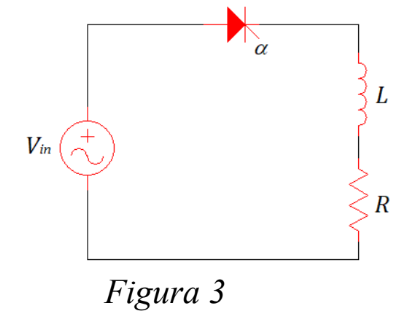
\includegraphics[width=0.45\textwidth]{ej3_rectificador_controlado_media_onda_circuito_figura3.png}
\caption{Rectificador Controlado de Media Onda}
\end{figure}

\subsection{Soluci\'on Anal\'itica}

Como primer paso se determina la constante de tiempo del circuito y su inverso,
que gobiernan la respuesta natural. F\'ormula general: $\tau = L/R$ y
$1/\tau = R/L$.

\begin{align*}
\tau &= \frac{0.045\Omega s}{34\Omega} = \boxed{1.32ms} \\
\frac{1}{\tau} &= \boxed{756\ \tfrac{1}{s}}
\end{align*}

A continuaci\'on, el \'angulo expresado en grados se convierte a su equivalente en
radianes. F\'ormula general: $\alpha_{rad} = \alpha_{grados}\cdot\dfrac{\pi}{180^\circ}$.

\begin{align*}
\alpha = 62^\circ\cdot\frac{\pi}{180^\circ} = \boxed{\tfrac{31}{90}\pi}
\end{align*}

A partir del \'angulo de disparo se obtiene el instante en que se activa el SCR.
F\'ormula general: $t_1 = \alpha/\omega$, con $\omega = 2\pi f = 120\pi\ \frac{rad}{s}$.

\begin{align*}
t_1 = \frac{\frac{31}{90}\pi\ rad}{120\pi\ \frac{rad}{s}} = \boxed{2.87ms}
\end{align*}

Seguidamente se calcula la impedancia de la carga y se expresa en forma polar.
F\'ormulas generales: $Z = R + j\omega L$, $|Z| = \sqrt{R^2 + (\omega L)^2}$ y
$\varphi = \tan^{-1}\!\left(\dfrac{\omega L}{R}\right)$.

\begin{align*}
Z &= 34\Omega + j(120\pi\,\tfrac{rad}{s})(0.045\Omega s) = \boxed{34\Omega + j17\Omega} \\
Z &= \boxed{38.0\Omega\angle 0.464r}
\end{align*}

Con esta impedancia se halla la corriente fasorial, de la cual proviene la
respuesta forzada del circuito. F\'ormula general:
$I = \dfrac{V_m\angle 0}{|Z|\angle\varphi}$.

\begin{align*}
I = \frac{220V\angle 0r}{38.0\Omega\angle 0.464r} = \boxed{5.79A\angle -0.464r}
\end{align*}

Por funci\'on general, la corriente queda planteada como la suma de la respuesta
forzada y la respuesta natural. F\'ormula general:
$i = I_m\,sen(\omega t - \varphi) + I_0\,e^{-(t-t_1)/\tau}$.

\begin{align*}
i = 5.79A\,Sen(120\pi t - 0.464r) + I_0 e^{-756(t-2.87\cdot10^{-3}s)}
\end{align*}

Evaluando la condici\'on inicial, con $t=2.87ms \rightarrow i=0$, se despeja la
constante $I_0$. F\'ormula general:
$0 = I_m\,sen(\omega t_1 - \varphi) + I_0 e^0 \Rightarrow I_0 = -I_m\,sen(\omega t_1 - \varphi)$.

\begin{align*}
0 &= 5.79A\,Sin(120\pi(2.87\cdot10^{-3}) - 0.464r) + I_0 e^{0} \\
I_0 &= \boxed{-3.35A}
\end{align*}

De igual manera, imponiendo la condici\'on final $t=t_e \rightarrow i=0$ se
plantea la ecuaci\'on del tiempo de extinci\'on. F\'ormula general:
$0 = I_m\,sen(\omega t_e - \varphi) + I_0 e^{-(t_e-t_1)/\tau}$.

\begin{align*}
0 = 5.79A\,Sen(120\pi t_e - 0.464r) - 3.35A\,e^{-756(t_e-2.87\cdot10^{-3}s)}
\end{align*}

Con condiciones iniciales de $8.33ms \le t_e \le 16.7ms$ se obtiene que
(calculadora, SHIFT+SOLVE, valor inicial sugerido
$X = (\pi+\varphi)/\omega = (\pi + 0.464)/(120\pi) \approx 9.56ms$):

\begin{align*}
t_e = \boxed{9.55ms}
\end{align*}

Por \'ultimo, este tiempo de extinci\'on se lleva a su equivalente angular.
F\'ormula general: $\beta = \omega\,t_e$.

\begin{align*}
\beta = (120\pi\,\tfrac{rad}{s})(9.55\cdot10^{-3}s) = \boxed{3.60\,rad}
\end{align*}

\subsection{Valores promedio y Eficaces de Tensiones y Corrientes}

De tensi\'on. Al ser media onda, el periodo de la se\~nal de salida es $2\pi$.
F\'ormula general:
$V_{DC} = \dfrac{1}{2\pi}\displaystyle\int_{\alpha}^{\beta} V_m\,sen\theta\,d\theta
= \dfrac{V_m}{2\pi}\left[-\cos\theta\right]_{\alpha}^{\beta}$.

\begin{align*}
V_{DC} &= \frac{1}{2\pi}\int_{\frac{31}{90}\pi}^{3.60} 220V\,Sen\theta\,d\theta
= \frac{220V}{2\pi}\left[-\Cos\theta\right]\Big|_{\frac{31}{90}\pi}^{3.6}
= \frac{220V}{2\pi}\left[-\Cos(3.6)+\Cos\!\left(\tfrac{31}{90}\pi\right)\right] \\
V_{DC} &= \boxed{47.8V}
\end{align*}

F\'ormula general:
$V_{RMS}^2 = \dfrac{1}{2\pi}\displaystyle\int_{\alpha}^{\beta} (V_m\,sen\theta)^2 d\theta
= \dfrac{V_m^2}{2\pi}\left[\dfrac{\theta}{2}-\dfrac{sen(2\theta)}{4}\right]_{\alpha}^{\beta}$.

\begin{align*}
V_{RMS}^2 &= \frac{(220V)^2}{2\pi}\int_{\frac{31}{90}\pi}^{3.60}(\Sen\theta)^2 d\theta
= \frac{(220V)^2}{2\pi}\left[\frac{\theta}{2}-\frac{\Sen(2\theta)}{4}\right]\Bigg|_{\frac{31}{90}\pi}^{3.6} \\
V_{RMS}^2 &= \frac{(220V)^2}{2\pi}\left[\left(\frac{3.6}{2}-\frac{\Sen(2(3.6))}{4}\right)-\left(\frac{\frac{31}{90}\pi}{2}-\frac{\Sen(2(\frac{31}{90}\pi))}{4}\right)\right] \\
V_{RMS} &= \sqrt{9766} = \boxed{98.8V}
\end{align*}

De corriente. La corriente solo existe entre $t_1$ y $t_e$ y se repite cada
$T = 1/60 = 16.67ms$. F\'ormula general:
$I_{DC} = \dfrac{1}{T}\displaystyle\int_{t_1}^{t_e} i(t)\,dt$ con $1/T = 60$.

\begin{align*}
I_{DC} &= 60\int_{2.87ms}^{9.55ms}\left(5.79A\,Sen(120\pi t - 0.464r) - 3.35A\,e^{-756(t-2.87ms)}\right)dt \\
I_{DC} &= \boxed{1.41A}
\end{align*}

F\'ormula general:
$I_{RMS}^2 = \dfrac{1}{T}\displaystyle\int_{t_1}^{t_e} i^2(t)\,dt$.

\begin{align*}
I_{RMS}^2 &= 60\int_{2.87ms}^{9.55ms}\left(5.79A\,Sen(120\pi t - 0.464r) - 3.35A\,e^{-756(t-2.87ms)}\right)^2 dt = 5.99A^2 \\
I_{RMS} &= \boxed{2.45A}
\end{align*}

\subsection{Potencias activa y aparente}

F\'ormulas generales: $P = I_{RMS}^2\,R$, \quad $S = V_{s,RMS}\,I_{RMS}$ con
$V_{s,RMS} = V_m/\sqrt{2} = 220V/\sqrt{2} = 156V$, \quad $P_{DC} = V_{DC}\,I_{DC}$.

\begin{align*}
P &= (2.45A)^2(34\Omega) = \boxed{204W} \\
S &= (156V)(2.45A) = \boxed{382VA} \\
P_{DC} &= (47.8V)(1.41A) = \boxed{67.4W}
\end{align*}

\subsection{Par\'ametros de rendimiento}

F\'ormulas generales: $fp = P/S$, \quad $\eta = P_{DC}/S$, \quad
$FR_V = \dfrac{\sqrt{V_{RMS}^2 - V_{DC}^2}}{V_{DC}}$, \quad
$FR_I = \dfrac{\sqrt{I_{RMS}^2 - I_{DC}^2}}{I_{DC}}$.

\begin{align*}
fp &= \frac{204W}{382VA} = \boxed{0.534} \\
\eta &= \frac{67.4W}{382VA} = \boxed{0.176} \\
FR_V &= \frac{\sqrt{(98.8V)^2-(47.8V)^2}}{47.8V} = \boxed{1.81} \\
FR_I &= \frac{\sqrt{(2.45A)^2-(1.41A)^2}}{1.41A} = \boxed{1.42}
\end{align*}

\subsection{Dibujo de se\~nales}

\subsubsection{Definiciones}

La se\~nal del voltaje de salida, definida en un periodo, est\'a dada por:
\begin{align*}
v_{o(t)} = \begin{cases} 220V\,Sen(120\pi t) & \text{si } 2.87\,ms \le t \le 9.55\,ms \\ 0 & \text{si } 0 \le t < 2.87\,ms \ \wedge\ 9.55\,ms < t \le 16.7\,ms \end{cases}
\end{align*}

Mientras que la funci\'on de corriente definida en el tiempo es:
\begin{align*}
i_{o(t)} = \begin{cases} 5.79A\,Sen(120\pi t - 0.464) - 3.35A\,e^{-756(t-2.87\cdot10^{-3})} & \text{si } 2.87ms \le t \le 9.55ms \\ 0 & \text{si } 0 \le t < 2.87ms \ \wedge\ 9.55ms < t \le 16.7ms \end{cases}
\end{align*}

\subsubsection{C\'odigo}

Se presenta el c\'odigo realizado en MatLAB para desarrollar las gr\'aficas
pertinentes, empezando con la de voltaje:

\begin{lstlisting}[language=Matlab, caption={C\'odigo, Voltaje}, label={lst:ej3vo}]
t = linspace(0, 1/60, 4000); t1 = 2.87e-3; te = 9.55e-3;
vo = 220*sin(120*pi*t) .* (t>=t1 & t<=te);
plot(t, vo, 'b', 'LineWidth', 1.5); grid on;
xlabel('Tiempo [s]'); ylabel('Voltaje [V]'); legend('vo(t)');
title('Tension de salida del rectificador');
\end{lstlisting}

Y tambien la de corriente:

\begin{lstlisting}[language=Matlab, caption={C\'odigo, Corriente}, label={lst:ej3io}]
t = linspace(0, 1/60, 4000); t1 = 2.87e-3; te = 9.55e-3;
io = (5.79*sin(120*pi*t-0.464) - 3.35*exp(-756*(t-t1))) .* (t>=t1 & t<=te);
plot(t, io, 'r', 'LineWidth', 1.5); grid on;
xlabel('Tiempo [s]'); ylabel('Corriente [A]'); legend('io(t)');
title('Corriente de salida del rectificador');
\end{lstlisting}

\subsubsection{Gr\'aficas resultantes}

\begin{figure}[H]
\centering
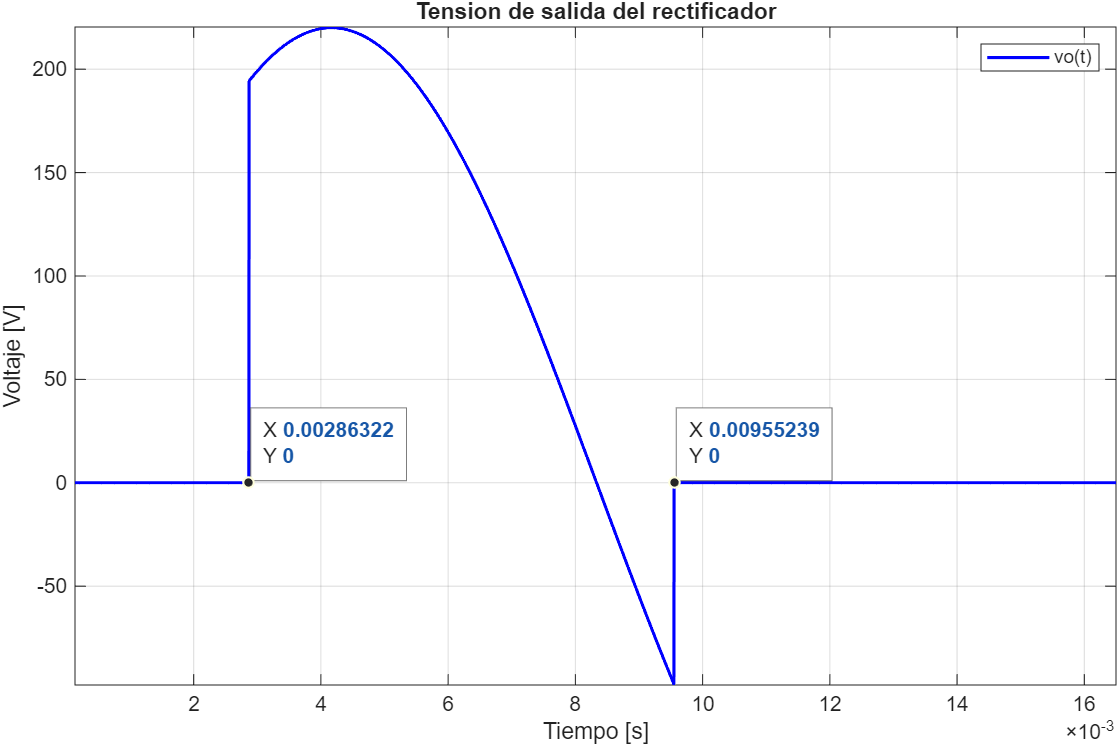
\includegraphics[width=0.8\textwidth]{ej3_tension_salida_vo_grafica_matlab_alpha62.png}
\caption{Tensi\'on de salida del rectificador}
\end{figure}

\begin{figure}[H]
\centering
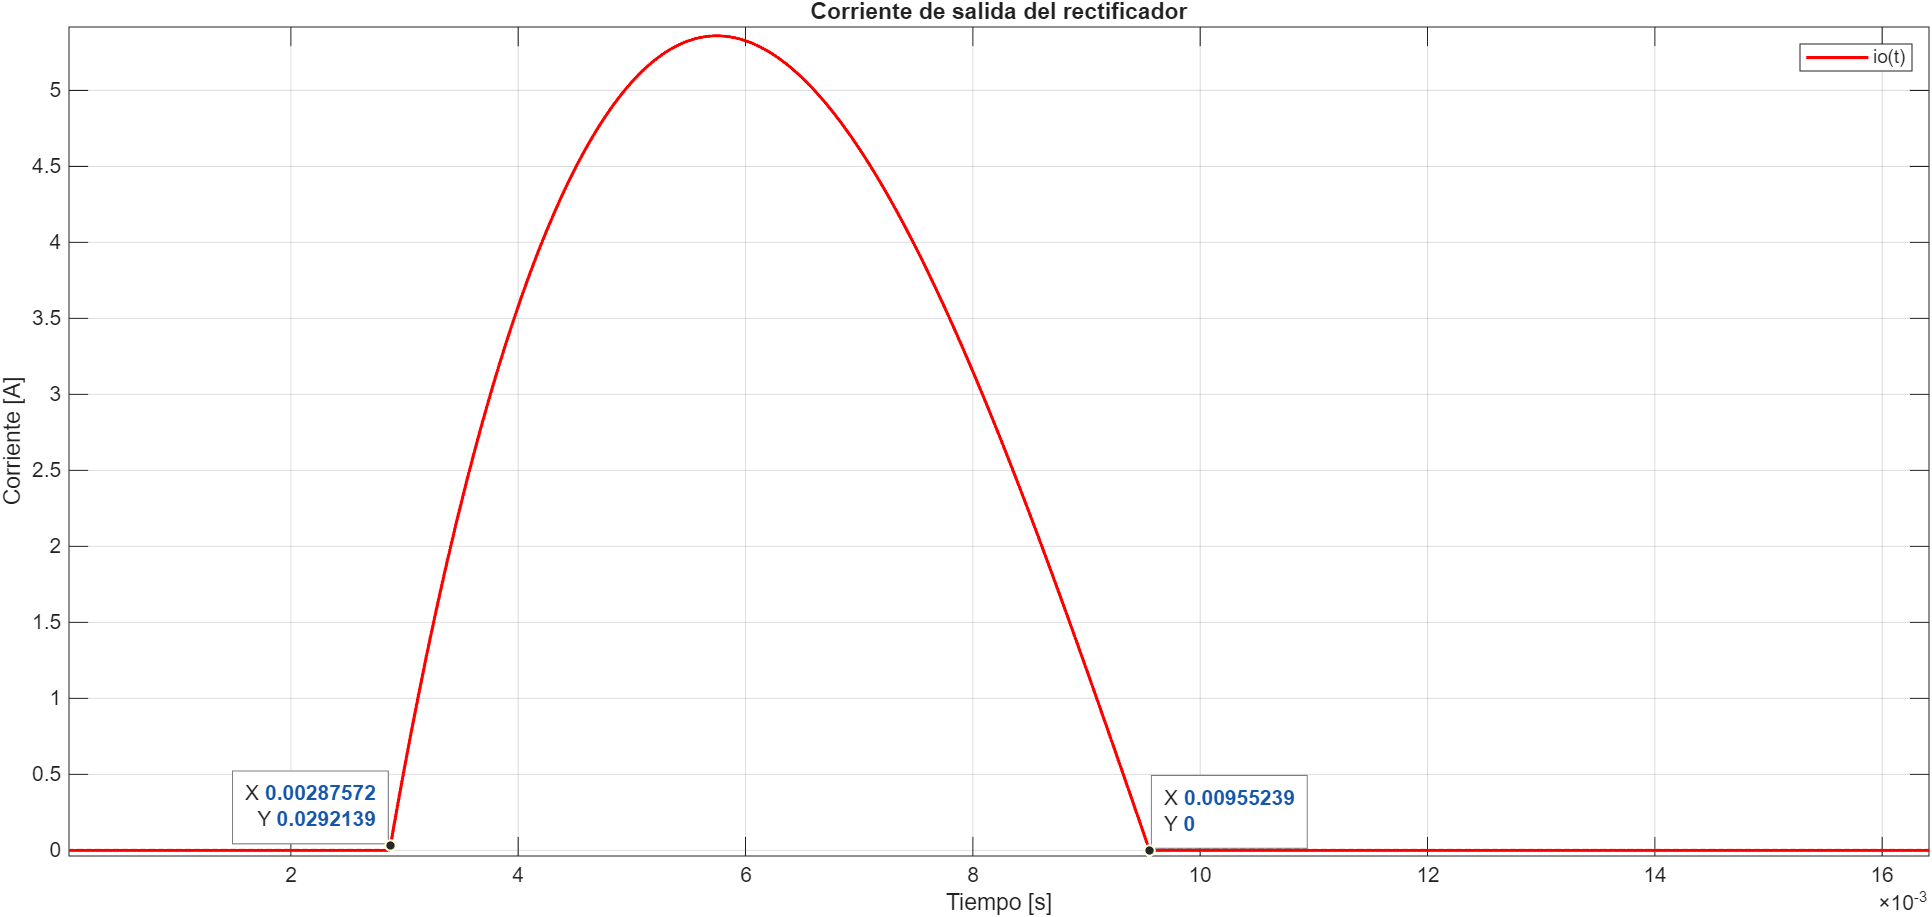
\includegraphics[width=0.9\textwidth]{ej3_corriente_salida_io_grafica_matlab_alpha62.png}
\caption{Corriente de salida del rectificador}
\end{figure}

\subsection{Simulaciones}

\subsubsection{Mediciones de tensiones y corrientes}

A continuaci\'on se presentan los datos observados en la simulaci\'on del
circuito propuesto:

\begin{figure}[H]
\centering
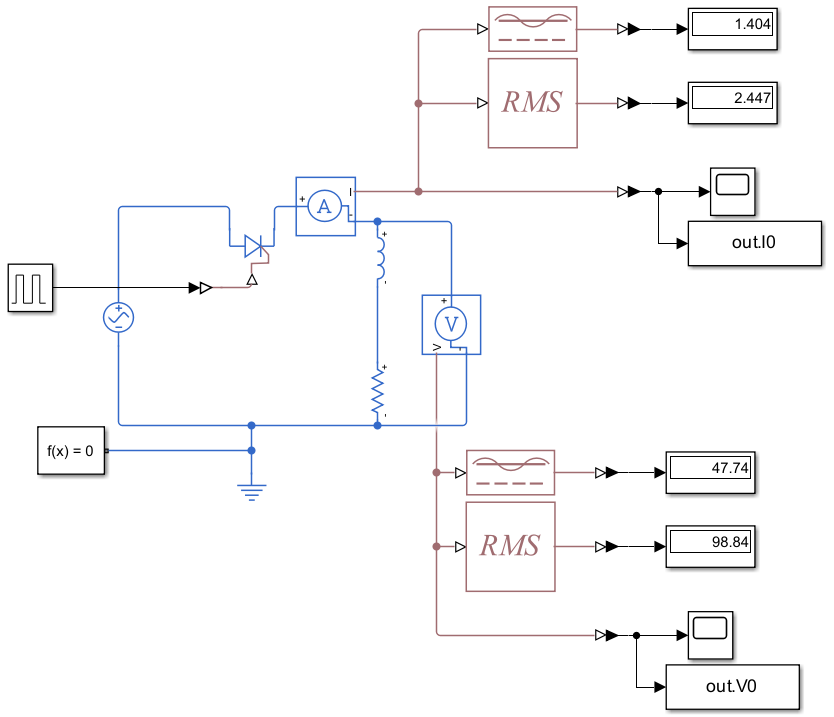
\includegraphics[width=0.75\textwidth]{ej3_simulacion_simscape_mediciones_media_onda_controlado.png}
\caption{Simulaci\'on rectificador controlado de Media Onda}
\label{fig:sim3}
\end{figure}

\subsubsection{Se\~nales de simulaci\'on}

Y sus respectivos gr\'aficos en los que se evidencian el retardo de 2.87 ms
correspondiente al \'angulo de disparo de $62^\circ$ y la extinci\'on de la
corriente en 9.55 ms, coincidentes con los valores obtenidos anal\'iticamente.

\begin{figure}[H]
\centering
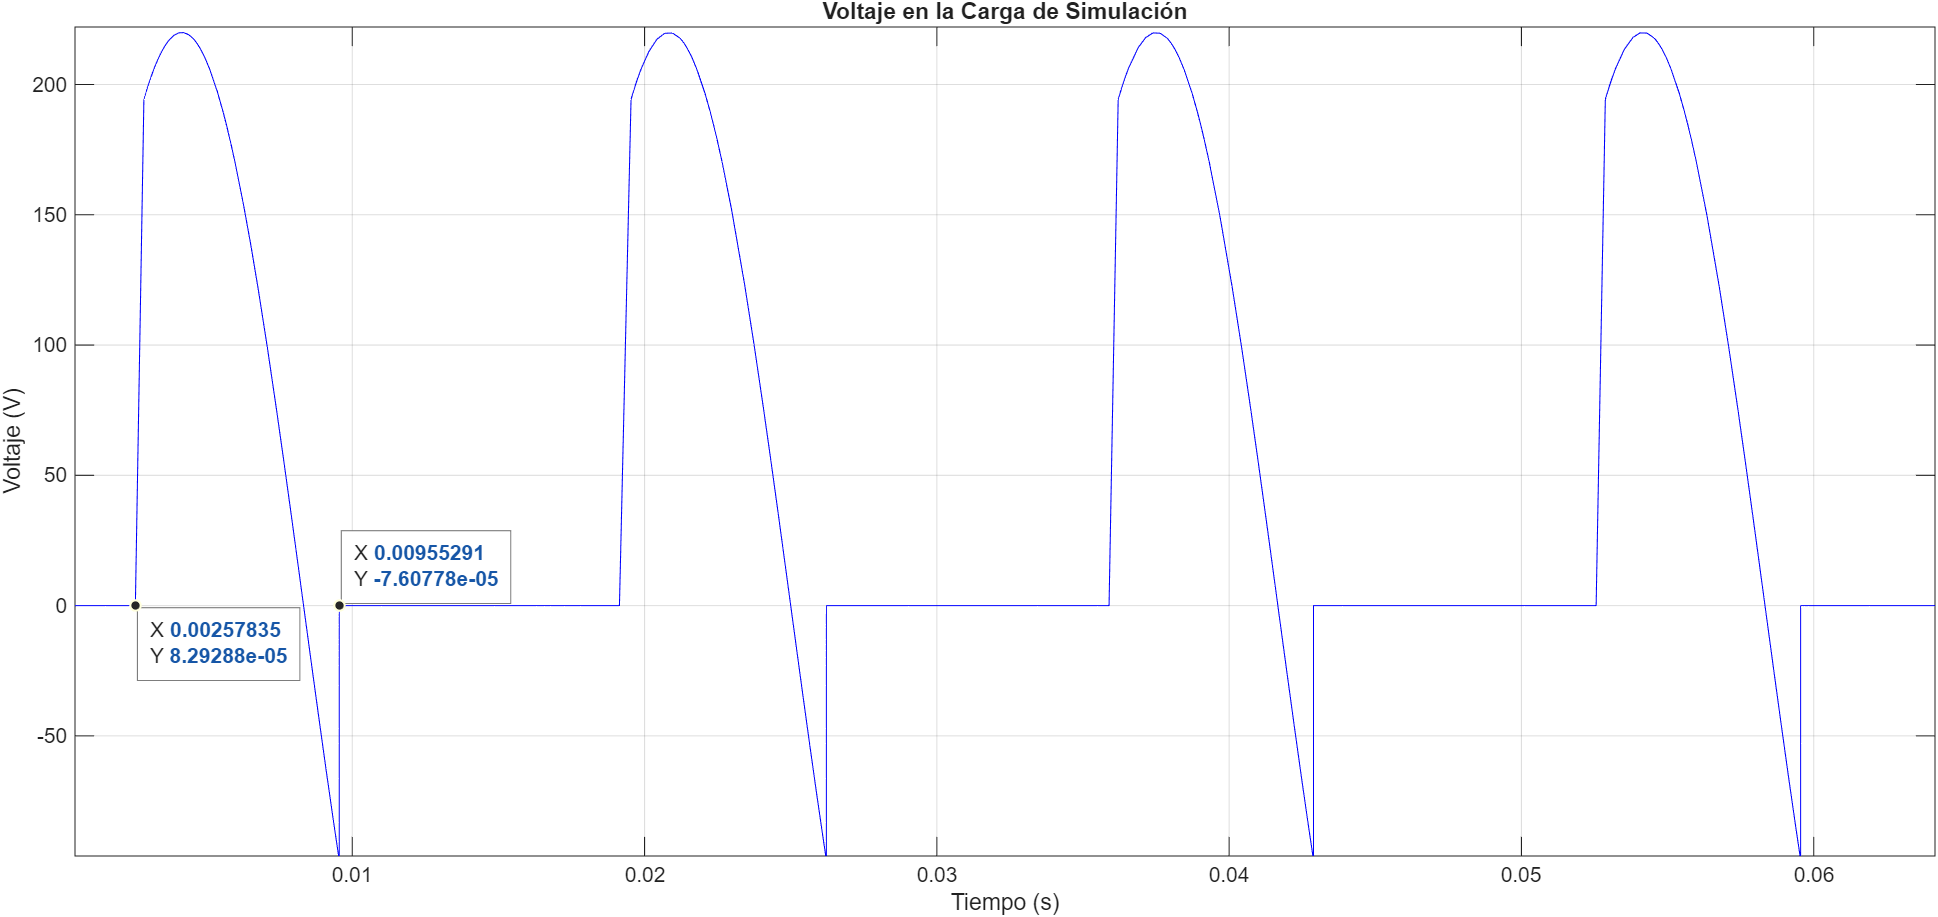
\includegraphics[width=0.95\textwidth]{ej3_simulacion_senal_voltaje_salida_vo_4_periodos.png}
\caption{Se\~nal de voltaje de salida Vo}
\end{figure}

\begin{figure}[H]
\centering
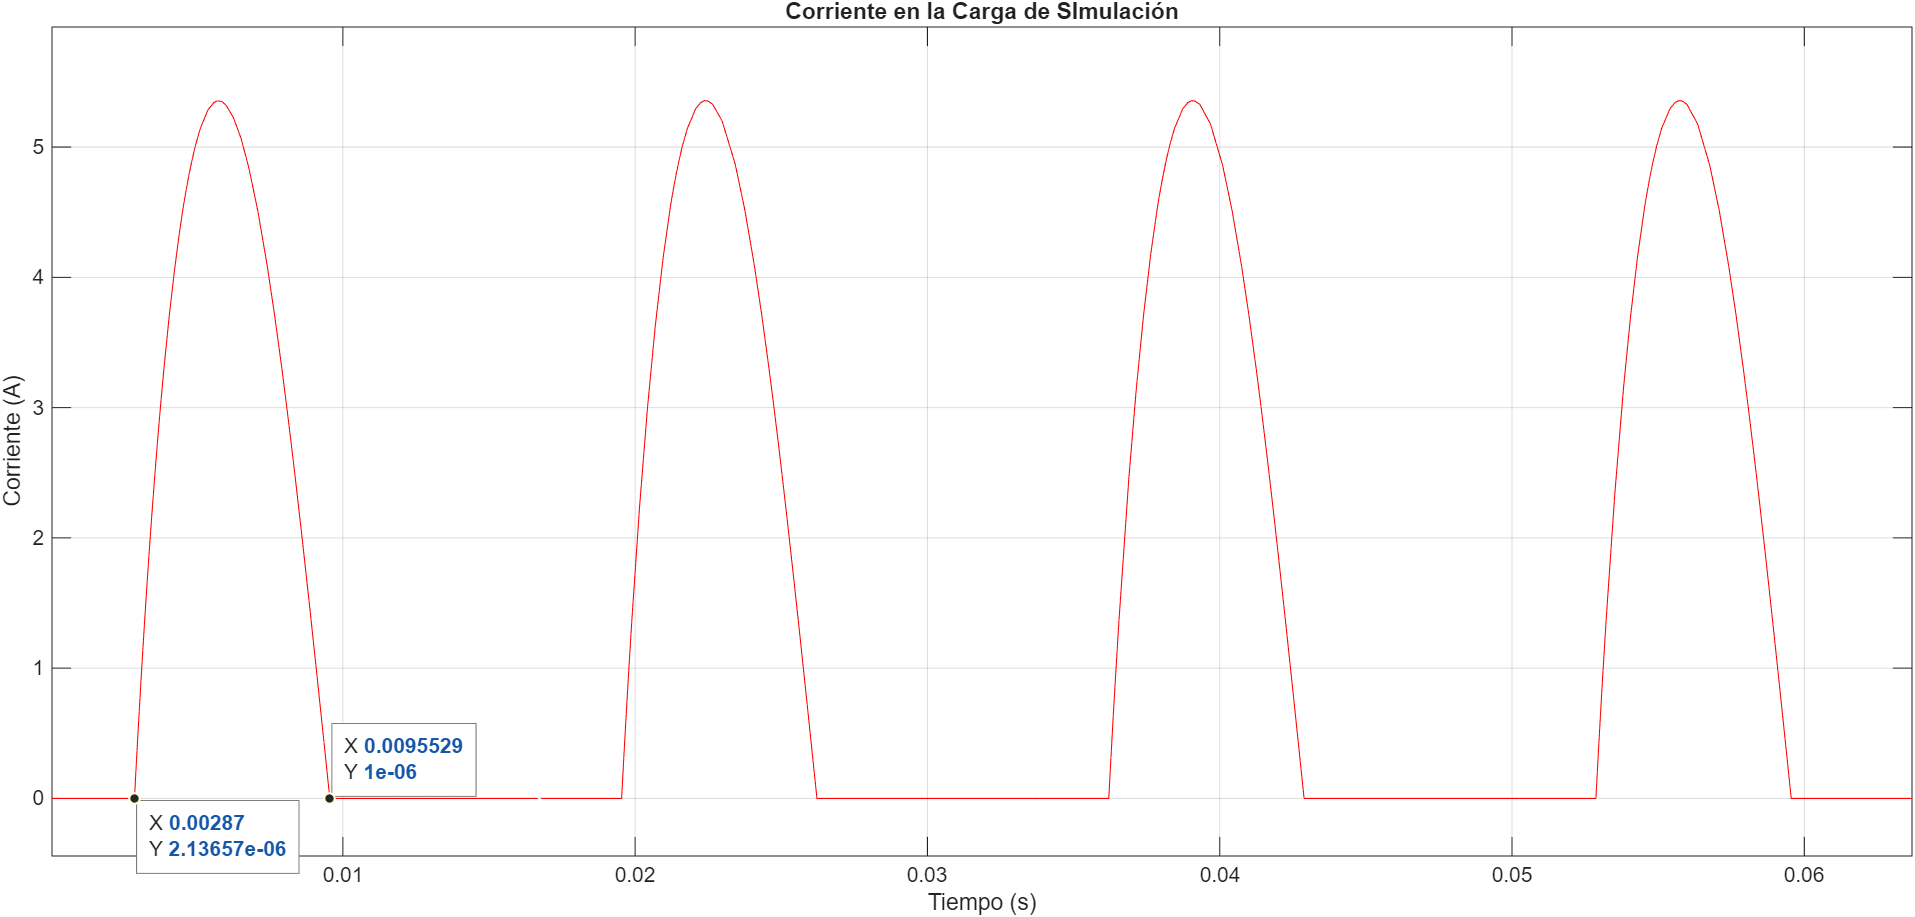
\includegraphics[width=0.95\textwidth]{ej3_simulacion_senal_corriente_salida_io_4_periodos.png}
\caption{Se\~nal de corriente de salida Io}
\end{figure}

\subsection{C\'alculos con los datos de simulaci\'on}

En la simulaci\'on se obtuvieron estos resultados (ver Figura~\ref{fig:sim3}):

\begin{align*}
V_{DC} = 47.74V \qquad V_{rms} = 98.84V \qquad I_{DC} = 1.404A \qquad I_{rms} = 2.447A
\end{align*}

Con estos datos se calculan los dem\'as par\'ametros as\'i (con las mismas
f\'ormulas generales de las secciones 3.4 y 3.5):

\begin{align*}
P &= (2.447A)^2(34\Omega) = \boxed{204W} \\
S &= (156V)(2.447A) = \boxed{382VA} \\
P_{DC} &= (47.74V)(1.404A) = \boxed{67.0W}
\end{align*}

\begin{align*}
fp &= \frac{204W}{382VA} = \boxed{0.534} \\
\eta &= \frac{67.0W}{382VA} = \boxed{0.175} \\
FR_V &= \frac{\sqrt{(98.84V)^2-(47.74V)^2}}{47.74V} = \boxed{1.81} \\
FR_I &= \frac{\sqrt{(2.447A)^2-(1.404A)^2}}{1.404A} = \boxed{1.43}
\end{align*}

\subsection{Comparaci\'on de resultados}

A continuaci\'on se muestra la tabla que compara los valores de simulaci\'on con
los datos de los c\'alculos anal\'iticos, tomando estos como referencia. F\'ormula
general del error:
$Error\,\% = \dfrac{|Valor_{calculado} - Valor_{simulaci\acute{o}n}|}{Valor_{calculado}}\times 100$.

\begin{center}
\textbf{Tabla 3:} Comparaci\'on de Par\'ametros Calculados y Simulados

\medskip
\begin{tabular}{|l|c|c|c|}
\hline
\textbf{\textcolor{blue}{Par\'ametros}} & \textbf{\textcolor{blue}{Valor Calculado}} & \textbf{\textcolor{blue}{Valor de Simulaci\'on}} & \textbf{\textcolor{red}{Error \%}} \\ \hline
$t_1$ (ms) & 2.87 & 2.870 & 0.000 \\
$t_e$ (ms) & 9.55 & 9.553 & 0.030 \\
$V_{DC}$ (V) & 47.8 & 47.74 & 0.126 \\
$V_{RMS}$ (V) & 98.8 & 98.84 & 0.040 \\
$I_{DC}$ (A) & 1.41 & 1.404 & 0.426 \\
$I_{RMS}$ (A) & 2.45 & 2.447 & 0.122 \\
$P$ (W) & 204 & 204 & 0.000 \\
$S$ (VA) & 382 & 382 & 0.000 \\
$P_{DC}$ (W) & 67.4 & 67.0 & 0.593 \\
$fp$ & 0.534 & 0.534 & 0.000 \\
$\eta$ & 0.176 & 0.175 & 0.568 \\
$FR_V$ & 1.81 & 1.81 & 0.000 \\
$FR_I$ & 1.42 & 1.43 & 0.704 \\ \hline
\end{tabular}
\end{center}

\end{document}
